\subparagraph*{Submission : }
\textit{Do the same as Step 6 when the conversion rates are not stationary. Adopt a sliding-window approach.}\\

The goal is the same of the previous problem, but in this case we are in a non-stationary environment, meaning that we have to introduce the seasonality. It is required to use a sliding-window approach.

Implementation: \textit{n7.py}
\subsection*{Basic knowledge}
\subparagraph*{Sliding Window Thompson Sampling (SWTS)} 
The Sliding Window Thompson Sampling is an alternative to the classical Thompson Sampling algorithm that is susceptible to changes. The main difference is the introduction of a parameter, the sliding window, of length $\tau\in \mathbb{N}$ such that the algorithm, at every round $t$, takes into account only the rewards obtained in the last $\tau$ rounds. Based on these realizations, we apply a TS-based algorithm to decide which is the arm to pull in the next round. In particular, the expected value of each arm is coupled with a posterior distribution from which we draw samples, and the arm with the highest value is the next arm to play.\\

\underline{\textit{Pseudocode}}\\
1. At every time $t$ for every arm $a$:

\hspace{2em}$\tilde{\theta_{a}} \leftarrow Sample(\mathbb P(\mu_{a}=\theta_{a}))$ \\

2. At every time $t$ play arm $a_{t}$ such that 

\hspace{2em}$a_{t} \leftarrow \argmax_{a \in A} \left\{ \tilde{\theta_{a}}  \right\} $ \\

3.  Update beta distribution of arm $a_{t}$

\hspace{2em}if $t\leq\tau$: $(\alpha_{a_{t}}, \beta_{a_{t}}) \leftarrow (\alpha_{a_{t}}, \beta_{a_{t}}) + (x_{a_{t},t}, 1 - x_{a_{t},t})$ 

\hspace{2em}if $\tau<t$:	$(\alpha_{a_{t}}, \beta_{a_{t}}) \leftarrow \max \left\{(1,1), (\alpha_{a_{t}}, \beta_{a_{t}}) + (x_{a_{t},t}, 1 - x_{a_{t},t}) - (x_{a_{t-\tau},t-\tau}, 1 - x_{a_{t-\tau},t-\tau})    \right\}$

\subsection*{Strategy}
The strategy is the same of the previous submission with the introduction of the seasonality. We use two learner that will retrieve the optimal superarm describing the couple of prices for the two items. One learner is the classical Thompson Sampling, the same used in the previous submission, while the other one is the Sliding Window Thompson Sampling. The size of the window used for the SWTS is computed as the $\sqrt{days * avgDailyCustomer} * \alpha$, where $days$ is the time horizon, $avgDailyCustomer = 1000$ is the normalizing factor used to compute the daily customer instances and $\alpha = 30 $ is a multiplicative factor empirically computed. Regarding the matching phase we do the same as the previous submission using a Promo-Category UCB learner for every superarm. In order to deal with seasonality, at the beginning of every new season all the matching learners are reset.

\subparagraph{Implementation} 
\begin{itemize}
	\item Conversion rates change according to the season
	\item The time horizon is equally divided into three seasons
	\item Candidates for the \textit{Racing Skis} are: \{2110.0, 1900.0, 2420.0, 2690.0\}
	\item Conversion rate associated with the first item is not known
	\item Candidates for the \textit{Racing Ski Helmet} are: \{360.0, 410.0, 530.0, 600.0\}
	\item Conversion rate associated with the second item is not known
	\item Optimal promotion-category assignment need to be learnt
\end{itemize}
\subparagraph{Optimal strategy}
The computation of the optimal strategy is the same performed in the previous submission but is calculated three times, taking into account the three seasons.
\begin{center}
	\begin{tabular}{|c|p{4cm}|p{4cm}|p{4cm}|} 
	\hline
	Season & \textit{Racing Skis optimal price} & \textit{Racing Ski Helmet} optimal price & Optimal promo-category matching \\ \hline
	\multirow{4}{*}{Spring-Summer} & \multirow{4}{*}{1900.0} & \multirow{4}{*}{410.0} & Sport addicted: P$_0$ = 0\% (410.0)  \\ 
								   & 					   &                      & Gifted: P$_2$ = 20\% (328.0)          \\ 
								   & 					   &                      & Worried: P$_3$ = 30\% (287.0)         \\
								   & 					   &                      & Amateur: P$_1$ = 10\% (369.0)         \\ \hline
	\multirow{4}{*}{Autumn} & \multirow{4}{*}{2690.0} & \multirow{4}{*}{530.0}  & Sport addicted: P$_1$ = 10\% (477.0)\\ 
								   & 					   &                      & Gifted: P$_3$ = 30\% (371.0)         \\ 
								   & 					   &                      & Worried: P$_2$ = 20\% (424.0)         \\
								   & 					   &                      & Amateur: P$_0$ = 0\% (530.0)         \\ \hline
	\multirow{4}{*}{Winter} & \multirow{4}{*}{2420.0} & \multirow{4}{*}{600.0}  & Sport addicted: P$_3$ = 30\% (420.0)\\ 
								   & 					   &                      & Gifted: P$_1$ = 10\% (540.0)         \\ 
								   & 					   &                      & Worried: P$_2$ = 20\% (480.0)         \\
								   & 					   &                      & Amateur: P$_0$ = 0\% (600.0)          \\ \hline
	\end{tabular}
\end{center}

\subsection*{Results}
\begin{center}
	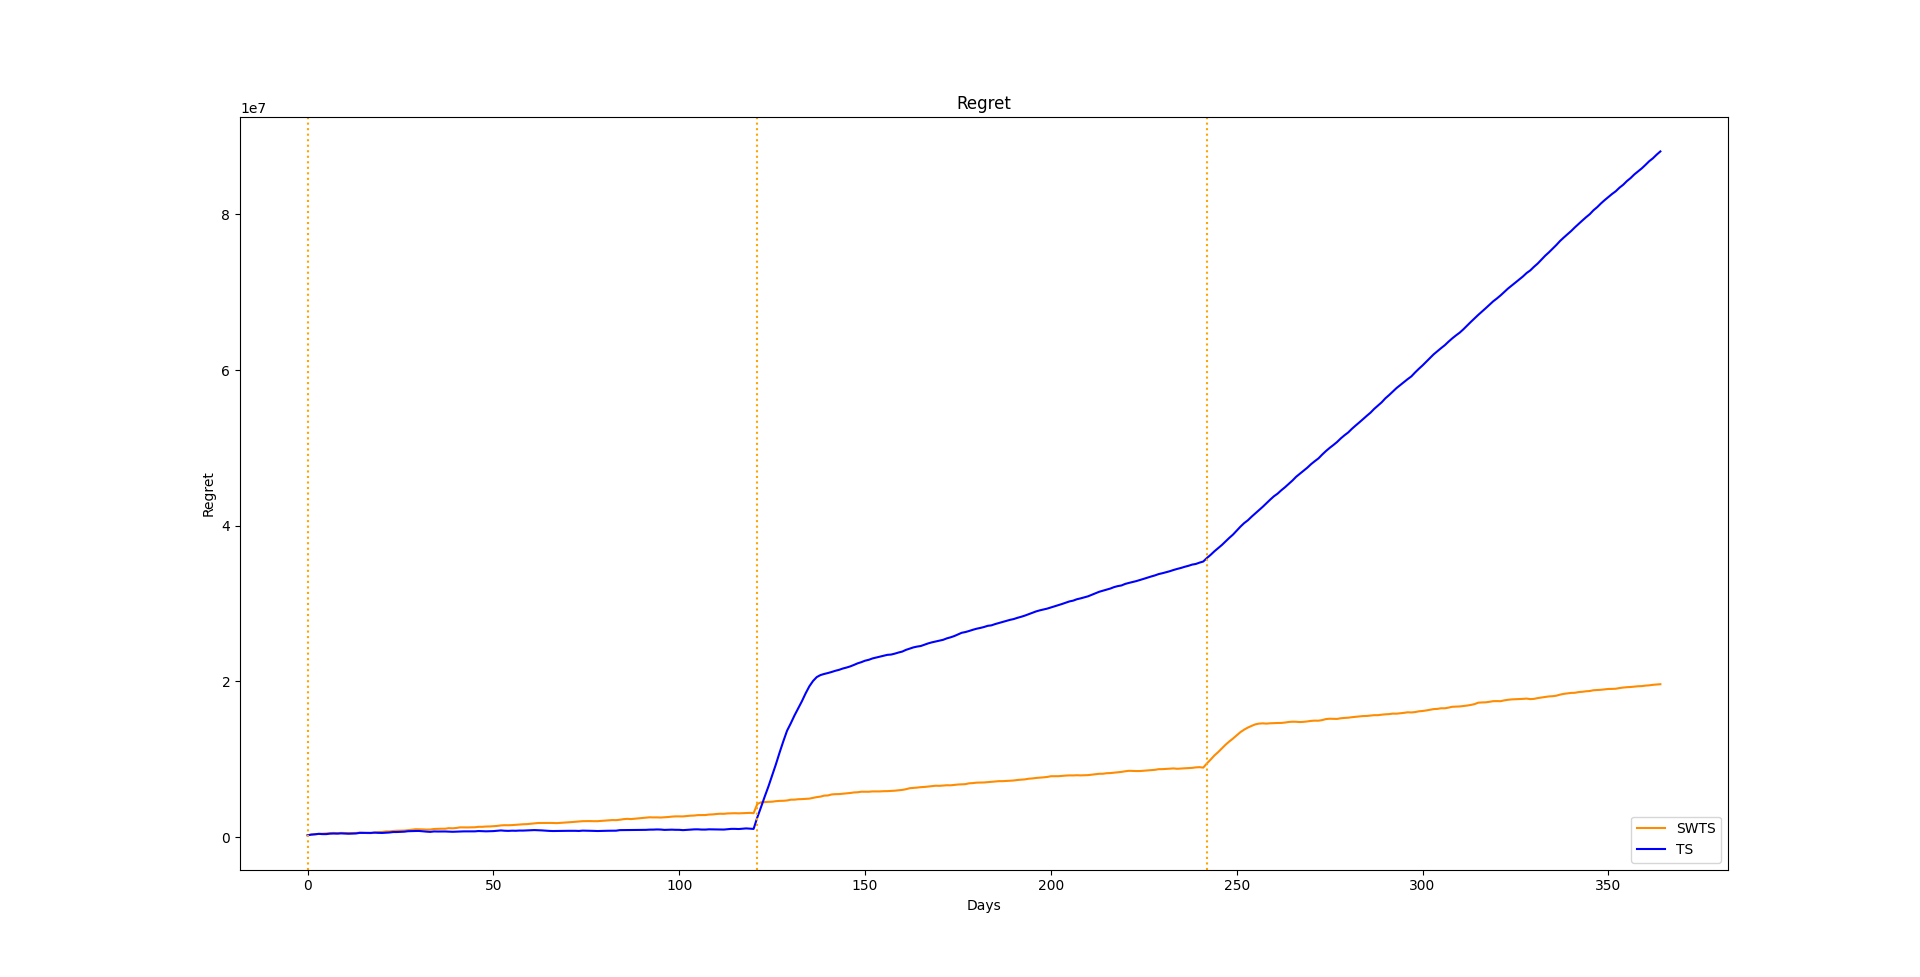
\includegraphics[scale=0.30]{Images/n7}
\end{center}
Days: 365\\
Number of seasons: 3 \\
Season length : $|365/3| = 122 $ days\\
Experiments number: 3 \\
Starting delay of the Promo-Category UCB Matching: 1000 clients\\
SWTS window size : $\sqrt{365 * 1000} * 30$\\
\subsection*{Considerations}
We can observe that in the first season the TS perform better since it has a complete knowledge of the collected samples, while the SWTS discards the older samples. However, when the conversion rates change, due to the change of the season, with the sliding window approach the newer samples become predominant. Thus, the algorithm changes its behaviour adapting the solution to the new season. We can note that the cumulative regret for the SWTS is about 4 times less than the TS. 